
\chapter{Theorem of mean value; indeterminant forms}


%105. 
\section{Rolle's Theorem}
\label{sec:105}

Let $y = f(x)$ be a continuous single-valued function of $x$, 
vanishing for $x = a$ and $x = b$, and suppose that $f'(x)$ 
changes continuously when $x$ varies from $a$ to $b$. 
The function will then be represented graphically by a 
continuous curve as in the figure. Geometric intuition 
shows us at once that for at least one value of $x$ 
between $a$ and $b$ the tangent is parallel to the $x$-axis 
(as at P); that is, the slope is zero. 

\begin{figure}[h!]
%\begin{tabular}{cc}
\begin{minipage}{\textwidth}
\begin{center}
%\vspace{1.0 cm}
%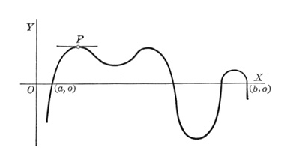
\includegraphics[height=3cm,width=6cm]{rolles-theorem.eps}
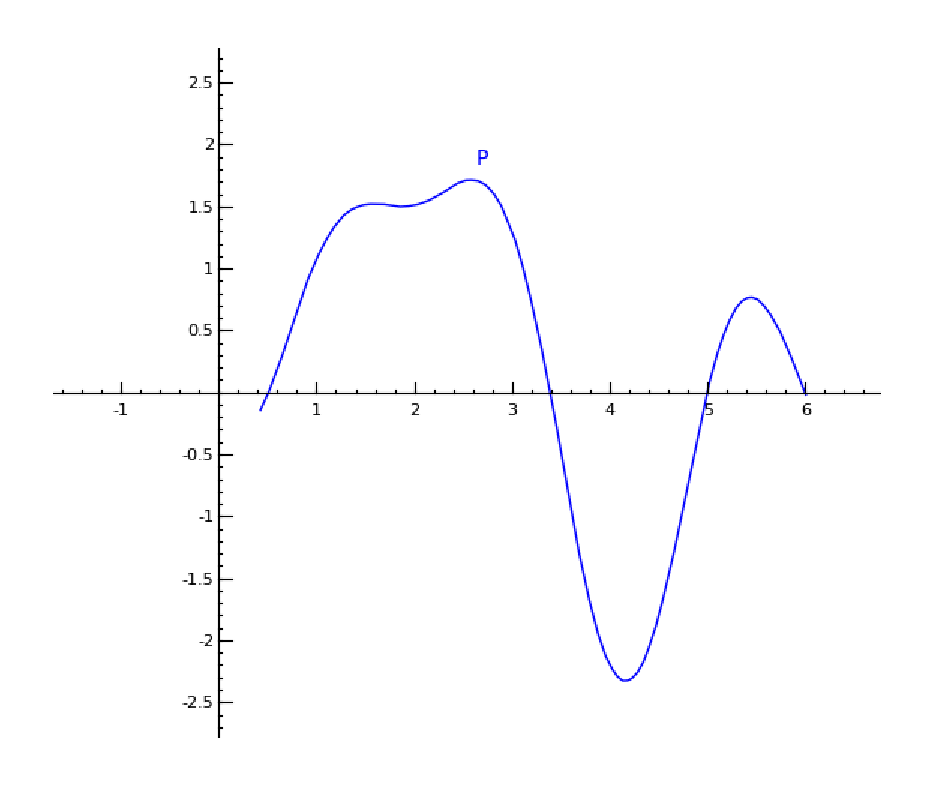
\includegraphics[height=5cm,width=9cm]{rolles-theorem3.eps}
\end{center}
\end{minipage}
%\caption{Scan of Granville's graphic illustrating Rolle's theorem.}
\caption{Geometrically illustrating Rolle's theorem.}
\label{fig:rolles-theorem}
\end{figure}

\noindent
This illustrates 

Rolle's Theorem:
{\it If $f(x)$ vanishes when $x = a$ and $x = b$, and $f(x)$ and 
$f'(x)$ are continuous for all values of $x$ from $x = a$ to 
$x = b$, then $f'(x)$ will be zero for at least one value of 
$x$ between $a$ and $b$.}
\index{Rolle's Theorem}

This theorem is obviously true, because as x 
increases from $a$ to $b$, $f(x)$ cannot always increase or 
always decrease as $x$ increases, since $f(a) = 0$ and $f(b) = 0$. 
Hence for at least one value of $x$ between $a$ and $b$, 
$f(x)$ must cease to increase and begin to decrease, 
or else cease to decrease and begin to increase; and for 
that particular value of $x$ the first derivative must 
be zero (see \S \ref{sec:81}). %§ 81, p. 108).

That Rolle's Theorem does not apply when $f(x)$ or $f'(x)$ 
are discontinuous is illustrated as follows:

\begin{figure}[h!]
\begin{tabular}{cc}
%\begin{minipage}{\textwidth}
%\begin{center}
%\vspace{1.0 cm}
%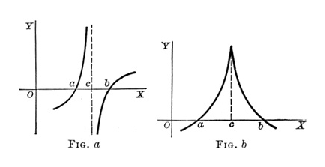
\includegraphics[height=3cm,width=6cm]{rolles-theorem2.eps}
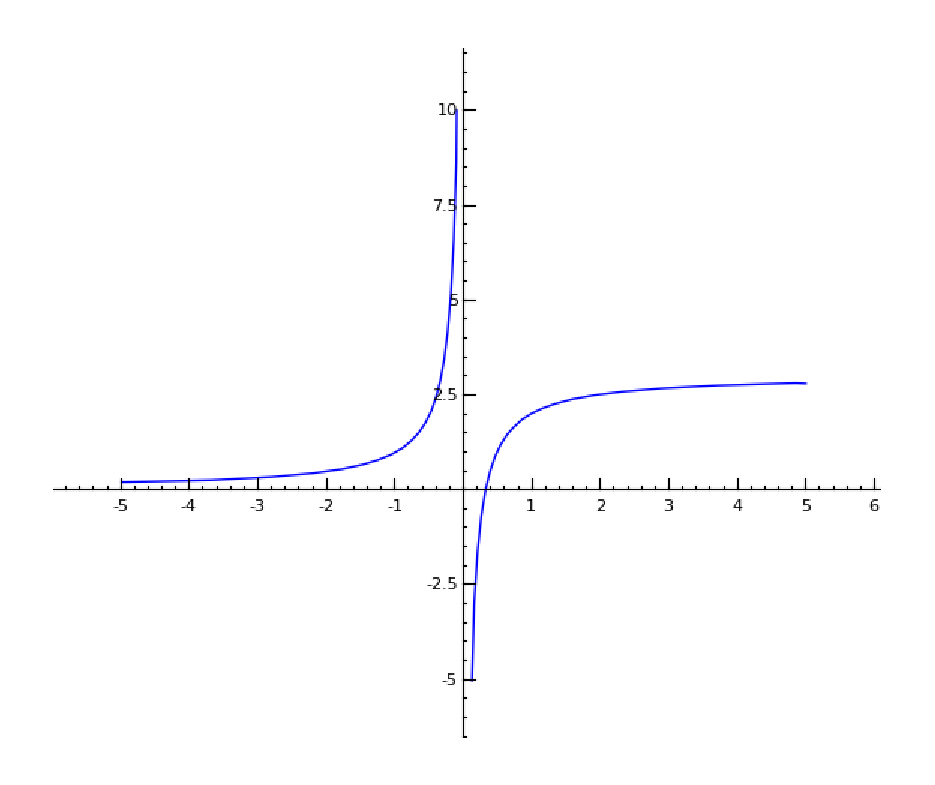
\includegraphics[height=5cm,width=5cm]{rolles-theorem4a.eps}
%\end{center}
%\end{minipage}
&
%\begin{minipage}{\textwidth}
%\begin{center}
%\vspace{1.0 cm}
%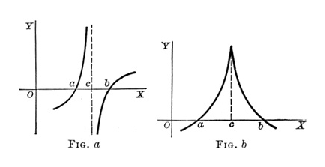
\includegraphics[height=3cm,width=6cm]{rolles-theorem2.eps}
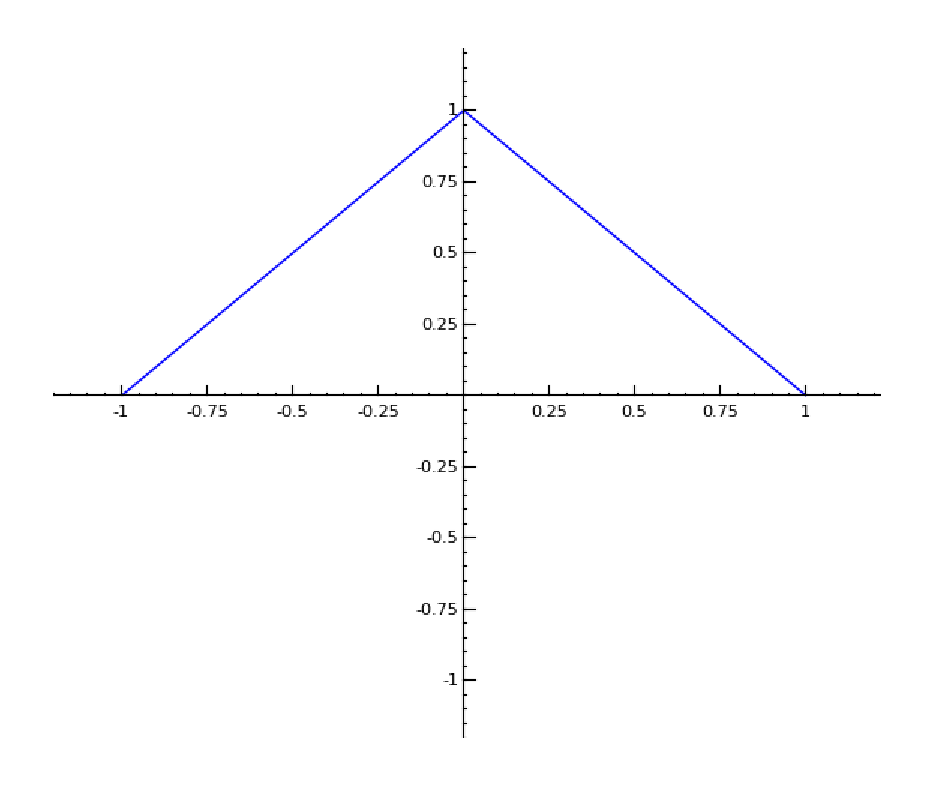
\includegraphics[height=5cm,width=5cm]{rolles-theorem4b.eps}
%\end{center}
%\end{minipage}
%\caption{Scan of Granville's graphic illustrating a counterexample to Rolle's theorem.}
\end{tabular}
\caption{Counterexamples to Rolle's theorem.}
\label{fig:rolles-theorem2}
\end{figure}

Figure \ref{fig:rolles-theorem2} (a) shows the graph of 
a function which is discontinuous (= $\infty$) for $x = c$, 
a value lying between $a$ and $b$. 
Figure \ref{fig:rolles-theorem2} (b) shows a continuous 
function whose first derivative is discontinuous (= $\infty$) 
for such an intermediate value $x = c$. In either case 
it is seen that at no point on the graph between $x = a$ 
and $x = b$ does the tangent (or curve) be,come parallel to 
the $x$-axis.

%106. 
\section{The Mean-value Theorem}
\label{sec:106}

Consider the quantity Q defined by the 
equation

\begin{equation}
%(A) 	
\frac{f(b) - f(a)}{b - a} = Q, 
\label{eqn:A-106}
\end{equation}
or

\begin{equation}
%(B) 	
f(b) - f(a) - (b - a)Q = 0.
\label{eqn:B-106}
\end{equation}
Let $F(x)$ be a function formed by replacing $b$ by $x$ 
in the left-hand member of (\ref{eqn:B-106}); that is,

\begin{equation}
%(C) 	
F(x) = f(x) - f(a) - (x - a)Q.
\label{eqn:C-106}
\end{equation}
From (\ref{eqn:B-106}), 	
$F(b) = 0$, and from (\ref{eqn:C-106}), $F(a) = 0$;
therefore, by Rolle's Theorem (see \S \ref{sec:105}), %p. 164 [§105]) 
$F'(x)$ must be zero for at least one value of $x$ between 
$a$ and $b$, say for $x_1$. But by differentiating (\ref{eqn:C-106}) we get
 
\[
 	F'(x) = f'(x) - Q.
\]
Therefore, since $F'(x_1) = 0$, then also 
$f'(x_1) - Q = 0$, and 	$Q = f'(x_1)$.
Substituting this value of Q in (\ref{eqn:A-106}), we get the 
Theorem of Mean Value\footnote{Also called the Law of the Mean.},

\begin{equation}
%(44) 	
\frac{f(b) - f(a)}{b - a} = f'(x_1),\ a < x_1 < b
\label{eqn:44-106}
\end{equation}
where in general all we know about $x_1$ is that it lies 
between $a$ and $b$.

\noindent
{\bf The Theorem of Mean Value interpreted Geometrically}. 

Let the curve in the figure be the locus of $y = f(x)$.


\begin{figure}[h!]
%\begin{tabular}{cc}
\begin{minipage}{\textwidth}
\begin{center}
%\vspace{1.0 cm}
%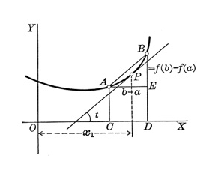
\includegraphics[height=3cm,width=5cm]{mean-value.eps}
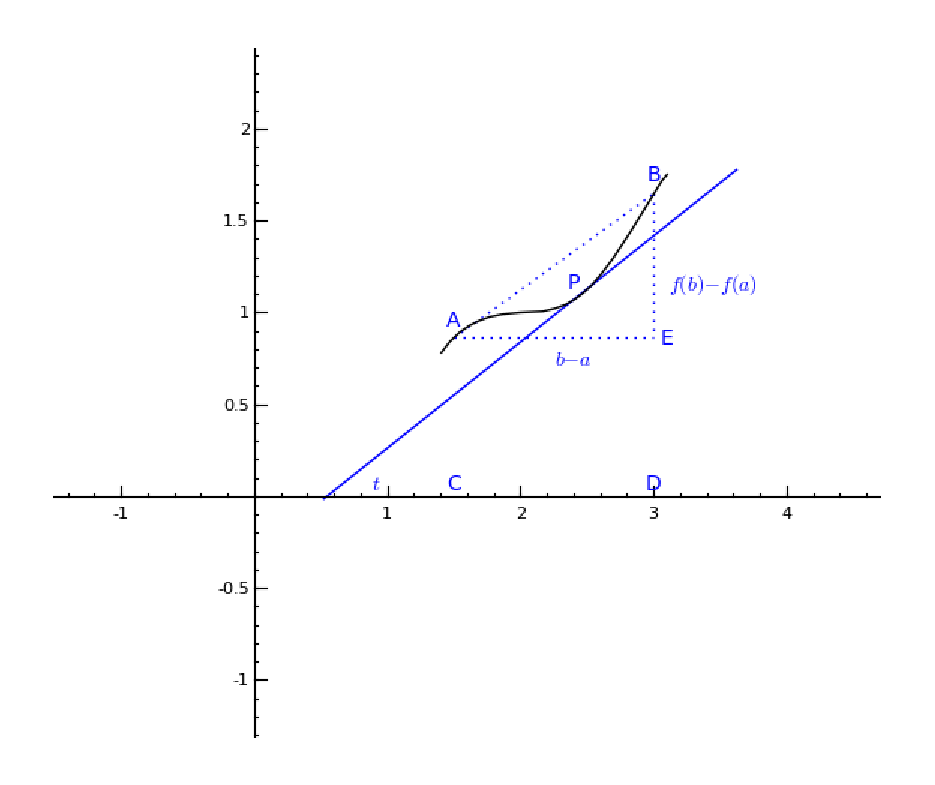
\includegraphics[height=5cm,width=8cm]{mean-value2.eps}
\end{center}
\end{minipage}
%\caption{Scan of Granville's graphic illustrating the Mean value theorem.}
\caption{Geometric illustration of the Mean value theorem.}
\label{fig:mean-value}
\end{figure}

Take $OC = a$ and $OD = b$; then $f(a) = CA$ and $f(b) = DB$, giving 
$AE = b - a$ and $EB = f(b) - f(a)$.
Therefore the slope of the chord AB is

\[
%(D) 	
\tan EAB = \frac{EB}{AE} = \frac{f(b) - f(a)}{b - a}.
\]
There is at least one point on the curve between A and B (as P) 
where the tangent (or curve) is parallel to the chord AB. 
If the abscissa of P is $x_1$ the slope at P is

\[
%(E) 	
\tan\, t = f'(x_1) = \tan\, EAB.
\]
Equating these last two equations, %(D) and (E), 
we get

\[  	
\frac{f(b) - f(a)}{b - a} = f'(x_1),
\]
which is the Theorem of Mean Value.
\index{Mean Value Theorem}

The student should draw curves (as the one in \S \ref{sec:105}), 
%on p. 164 [§105]) 
to show that there may be more than one such point in the 
interval; and curves to illustrate, on the other hand, 
that the theorem may not be true if $f(x)$ becomes discontinuous 
for any value of $x$ between $a$ and $b$ 
(see Figure \ref{fig:rolles-theorem2} (a)), %Fig. a, p. 164), 
or if $f'(x)$ becomes discontinuous 
(see Figure \ref{fig:rolles-theorem2} (b)). %Fig. b, p. 164).

Clearing (\ref{eqn:44-106}) of fractions, we may also write 
the theorem in the form

\begin{equation}
%(45) 	
f(b) = f(a) + (b - a)f'(x_1).
%\label{eqn:45-106}
\label{eqn:106-45}
\end{equation}
Let $b = a + \Delta a$; then $b - a = \Delta a$, and since $x_1$ is a 
number lying between $a$ and $b$, we may write
\[
  	x_1 = a + \theta \cdot \Delta a,
\]
where $\theta$ is a positive proper fraction. Substituting 
in (\ref{eqn:44-106}), we get another form of the 
Theorem of Mean Value.

\begin{equation}
%(46) 	
f(a + \Delta a) - f(a) = \Delta a f'(a + \theta \cdot \Delta a),
\ \ \ 0 < \theta < 1.
\label{eqn:46-106}
\end{equation}

%107. 
\section{The Extended Mean Value Theorem}
\index{Extended Mean Value Theorem}
\label{sec:107}

Following the method of the last section, 
let $R$ be defined by the equation

\begin{equation}
%(A) 	
f(b) - f(a) - (b - a)f'(a) - \frac{1}{2} (x - a)^2R = 0.
\label{eqn:A-107}
\end{equation}
Let $F(x)$ be a function formed by replacing $b$ by $x$ in the 
left-hand member of (\ref{eqn:A-106}); that is,

\begin{equation}
%(B) 	
F(x) = f(x) - f(a) - (x - a) f'(a) - \frac{1}{2} (x - a)^2 R.
\label{eqn:B-107}
\end{equation}
From (\ref{eqn:A-107}), $F(b) = 0$; and from (\ref{eqn:B-107}), 
$F(a) = 0$; therefore, by Rolle's Theorem, % (p. 164), 
at least one value of $x$ 
between $a$ and $b$, say $x_1$ will cause 
$F'(x)$ to vanish. Hence, since

\[
F'(x) = f'(x) - f'(a) - (x - a)R, 
\]
we get

\[
F'(x_1) = f'(x_1) - f'(a) - (x_1 - a)R = 0.
\]
Since $F'(x_1) = 0$ and $F'(a) = 0$, it is evident that $F'(x)$ 
also satisfies the conditions of Rolle's Theorem, so that 
its derivative, namely $F''(x)$, must vanish for at least one 
value of $x$ between $a$ and $x_1$, say $x_2$, and therefore 
$x_2$ also lies between $a$ and $b$. But
$F''(x) = f''(x) - R$; 
therefore $F''(x_2) = f''(x_2) - R = 0$,
and $R = f''(x_2)$.
Substituting this result in (\ref{eqn:A-107}), we get

\[
%(C) 	
f(b) = f(a) + (b - a)f'(a) + \frac{1}{2!} (b - a)^2 f''(x_2),
\ \ \ \ a < x_2 < b.
\]
In the same manner, if we define $S$ by means of the equation

\[
f(b) -f(a) - (b - a) f'(a) 
- \frac{1}{2!} (b - a)^2 f''(a) 
- \frac{1}{3!}(b - a)^2 f''(a) S = 0,
\]
we can derive the equation

\begin{equation}
%(D) 	
\begin{array}{ll} 
f(b) = f(a) & + (b - a)f'(a) + \frac{1}{2!} (b - a)^2 f''(a) \\ 
& + \frac{1}{3!} (b - a)^3 f'''(x_3), a < x_3 < b ,
\end{array}
\label{eqn:107-D}
\end{equation}
where $x_3$ lies between $a$ and $b$.
By continuing this process we get the general result,

\[
%(E) 	
\begin{array}{ll} 
f(b) = f(a) & 
+ \frac{(b - a)}{1!}f'(a) + \frac{(b - a)^2}{2!}f''(a) \\ 
& + \frac{(b - a)^3}{3!}f'''(a) + \cdots 
+ \frac{(b - a)^{(n - 1)}}{(n - 1)!}f^{(n - 1)} (a) \\ 
& + \frac{(b - a)^n}{n!}f^{(n)} (x_1), \ \ \ \ a < x_1 < b, 
\end{array}
\]
where $x_1$ lies between $a$ and $b$. 
This equation %(E) 
is called the Extended Theorem of Mean Value\footnote{Also 
called the Extended Law of the Mean.}, or Taylor's formula.
\index{Taylor's formula}

\section{Exercises}

Examine the following functions for maximum and minimum values, 
using the methods above.

\begin{enumerate}
%1.
\item
$y=3x^4-4x^3+1$

Ans.
$x=1$ is a min., $y=0$; $x=0$ gives neither.

%2
\item
$y=x^3-6x^2+12x+48$

Ans.
$x=2$ gives neither.

%3
\item
$y=(x-1)^2(x+1)^3$

Ans.
$x=1$ is a min., $y=0$;
$x=1/5$ is a max;
$x=-1$ gives neither.


%4
\item
Investigate $y=x^5-5x^4+5x^3-1$ at $x=1$ and $x=3$.

%5
\item
Investigate $y=x^3-3x^2+3x+7$ at $x=1$.

%6
\item
Show the if the first derivative of $f(x)$ which does not vanish at
$x=a$ is of odd order $n$ then $f(x)$ is increasing or decreasing at
$x=a$, according to whether $f^{(n)}(a)$ is positive or negative.


\end{enumerate}


%108. 
\section{Maxima and minima treated analytically}
\label{sec:108}

By making use of the results of the last two sections we 
can now give a general discussion of maxima and minima of 
functions of a single independent variable.

Given the function $f(x)$. Let $h$ be a positive number as small 
as we please; then the definitions given in \S \ref{sec:82}, 
may be stated as follows:
If, for all values of $x$ different from $a$ in the interval $[a - h, a + h]$,

\begin{equation}
\label{eqn:108A}
%(A) 	
f(x)-f(a) =\ {\rm a\ negative\ number},
\end{equation}
then $f(x)$ is said to be a {\it maximum} when $x = a$.
\index{maximum}
If, on the other hand,

\begin{equation}
\label{eqn:108B}
%(B) 	
f(x)-f(a) =\ {\rm a\ positive\ number},
\end{equation}
then $f(x)$ is said to be a {\it minimum} when $x = a$.
\index{minimum}
Consider the following cases:

\begin{itemize}
\item[I] 
Let $f'(a) \ne 0$.
From (\ref{eqn:106-45}), [\S \ref{sec:106}], 
replacing b by x and transposing f(a),

\begin{equation}
\label{eqn:108C}
%(C) 	
f(x)-f(a) = (x-a)f'(x_1),\ \ \ \ a < x_1 < x,
\end{equation}
Since $f'(a) \ne 0$, and $f'(x)$ is assumed as continuous, $h$ 
may be chosen so small that $f'(x)$ will have the same sign 
as $f'(a)$ for all values of $x$ in the interval $[a - h, a + h]$. 
Therefore $f'(x_1)$ has the same sign as $f'(a)$ (Chap. \ref{ch:3}). 
But $x-a$ changes sign according as $x$ is less or greater than $a$. 
Therefore, from (\ref{eqn:108C}), the difference
$f(x)-f(a)$
will also change sign, and, by (\ref{eqn:108A}) and (\ref{eqn:108B}), 
$f(a)$ will be neither a maximum nor a minimum. This result 
agrees with the discussion in \S \ref{sec:82}, where it was 
shown that for all values of $x$ for which $f(x)$ is a maximum 
or a minimum, the first derivative $f'(x)$ must vanish.

\item[II]
Let $f'(a) = 0$, and $f''(a) \ne 0$.
From (\ref{eqn:108C}), replacing $b$ by $x$ and transposing $f(a)$,

\begin{equation}
\label{eqn:108D}
%(D) 	
f(x)-f(a) = \frac{(x - a)^2}{2!} f''(x_2),\ \ \ \ a < x_2 < x.
\end{equation}
Since $f''(a) \ne 0$, and $f''(x)$ is assumed as continuous, we 
may choose our interval $[a - h, a + h]$ so small that 
$f''(x_2)$ will have the same sign as $f''(a)$ (Chap. \ref{ch:3}). 
Also $(x-a)^2$ does not change sign. Therefore the second 
member of (\ref{eqn:108D}) will not change sign, and the difference
$f(x)-f(a)$
will have the same sign for all values of $x$ in the interval 
$[a - h, a + h]$, and, moreover, this sign will be the same 
as the sign of $f''(a)$.
It therefore follows from our definitions 
(\ref{eqn:108A}) and (\ref{eqn:108B}) that

\begin{equation}
\label{eqn:108E}
%(E) 	
f(a)\ {\rm is\ a\ maximum\ if}\ f'(a) = 0 \ {\rm and}\ f''(a) 
=\ {\rm a\ negative\ number};
\end{equation}
\begin{equation}
\label{eqn:108F}
%(F) 	
f(a)\ {\rm is\ a\ minimum\ if}\ f'(a) = 0 \ {\rm and}\ f''(a) 
=\ {\rm a\ positive\ number}
\end{equation}
These conditions are the same as (\ref{eqn:84-21}) and (\ref{eqn:84-22}), 
[\S \ref{sec:84}].

\item[III]
Let $f'(a) = f''(a) = 0$, and $f'''(a) \ne 0$.
From (\ref{eqn:107-D}), [\S \ref{sec:107}], replacing $b$ by $x$ 
and transposing $f(a)$,

\begin{equation}
\label{eqn:108G}
%(G) 	
f(x)-f(a) = \frac{1}{3!} (x-a)^3 f'''(x_3),\ \ \ \ a < x_3 < x.
\end{equation}
As before, $f'''(x_3)$ will have the same sign as $f'''(a)$. But 
$(x-a)^3$ changes its sign from $-$ to $+$ as $x$ increases through $a$. 
Therefore the difference
$f(x)-f(a)$
must change sign, and $f(a)$ is neither a maximum nor a minimum.

\item[IV]
Let $f'(a) = f''(a) = \cdots = f^{(n-l)}(a) = 0$, and $f^{(n)}(a) \ne 0$.
By continuing the process as illustrated in I, II, and III, it is 
seen that if the first derivative of $f(x)$ which does not vanish for 
$x = a$ is of even order ($= n$), then\footnote{As in \S \ref{sec:82}, 
a critical value $x = a$ is found by placing the first derivative equal 
to zero and solving the resulting equation for real roots.}

\begin{equation}
\label{eqn:108-47} 	
%(47)
f(a)\ {\rm is\ a\ maximum\ if}\ f^{(n)}(a) =\ {\rm a\ negative\ number};
\end{equation}
\begin{equation}
\label{eqn:108-48} 	
%(48)
f(a)\ {\rm is\ a\ minimum\ if}\ f^{(n)}(a) =\ {\rm a\ positive\ number}.
\end{equation}
If the firstderivative of $f(x)$ which does not vanish for $x = a$ is of odd order, 
then $f(a)$ will be neither a maximum nor a minimum.
\end{itemize}

\begin{example}
Examine $x^3-9x^2 + 24x-7$ for maximum and minimum values.

Solution. $f(x) = x^3-9x^2 + 24x-7$.
$f'(x) = 3x^2-18x + 24$.
Solving $3x^2-18x + 24 = 0$
gives the critical values $x = 2$ and $x = 4$. Thus
$f'(2) = 0$, and $f'(4) = 0$.
Differentiating again, 	$f''(x) = 6x-18$.
Since $f''(2) =-6$, we know from (\ref{eqn:108-47}) that $f(2) = 13$ is a maximum.
Since $f''(4) = + 6$, we know from (\ref{eqn:108-48}) that $f(4) = 9$ is a minimum.
\end{example}

\begin{example}
Examine $e^x + 2\cos(x) + e^{-x}$ for maximum and minimum values.

Solution. $f(x) = e^x + 2\cos(x) + e^{-x}$,
$f'(x) = e^x-2\sin x-e^{-x} = 0$, for $x = 0$
(and $x = 0$ is the {\it only} root of the equation $e^x-2\sin x-e^{-x} = 0$),
  	$f''(x) = e^x - 2\cos(x) + e^{-x} = 0$, for $x = 0$,
  	$f'''(x) = e^x+2\sin x-e^{-x} = 0$, for $x = 0$,
  	$f^{(4)}(x) = e^x + 2\cos(x) + e^{-x} = 4$, for $x = 0$.
Hence from (\ref{eqn:108-48}), $f(0) = 4$ is a minimum.
\end{example}

\section{Exercises}

Examine the following functions for maximum and minimum values, 
using the method of the last section.

\begin{enumerate}
\item
$3x^4-4x^3 + 1$.

Ans. 	$x = 1$ gives min. $= 0$; $x = 0$ gives neither.

\item
$x^3-6x^2 + 12x + 48$.

Ans.  	$x = 2$ gives neither.

\item
$(x-1)^2(x + 1)^3$.

Ans. $x = 1$ gives min. $= 0$;
$x = \frac{1}{5}$ gives max.;
$x = -1$ gives neither.

\item
Investigate $x^6-5x^4 + 5x^3-1$, at $x = 1$ and $x = 3$.

\item
Investigate $x^3-3x^2 + 3x + 7$, at $x = 1$.

\item
Show that if the first derivative of $f(x)$ which does not 
vanish for $x = a$ is of odd order ($= n$), then $f(x)$ is an increasing or 
decreasing function when $x = a$, according as $f^{(n)}(a)$ is positive or negative.
\end{enumerate}

%109. 
\section{Indeterminate forms}
\label{sec:109}

Some singularities are easy to diagnose.  Consider the function 
$\frac{\cos x}{x}$ at the point $x = 0$.  The function evaluates to 
$\frac{1}{0}$ and is thus discontinuous at that point.  Since the numerator
and denominator are continuous functions and the denominator vanishes while
the numerator does not, the left and right limits as $x \to 0$ do not 
exist.  Thus the function has an infinite discontinuity at the point
$x = 0$.  

\begin{figure}[h!]
%\begin{tabular}{cc}
\begin{minipage}{\textwidth}
\begin{center}
%\vspace{1.0 cm}
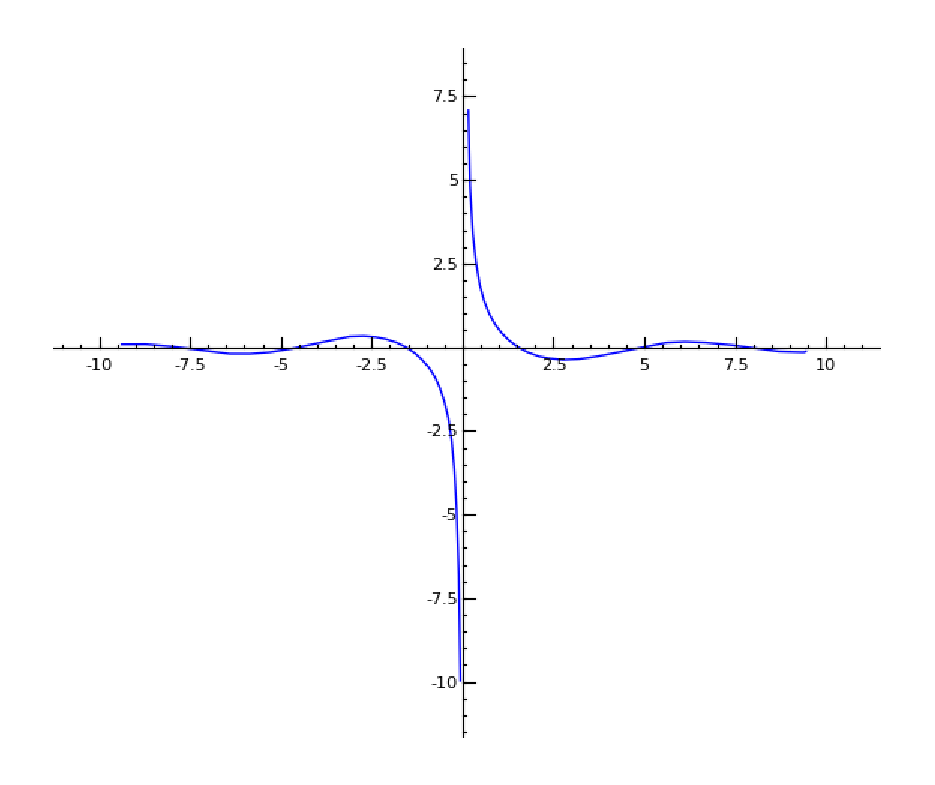
\includegraphics[height=5cm,width=10cm]{cosoverx.eps}
\end{center}
\end{minipage}
\caption{$\frac{\cos(x)}{x}$.}
\label{fig:cosoverx}
\end{figure}

\noindent
More generally, a function which is composed of continuous
functions and evaluates to $\frac{a}{0}$ at a point where $a \neq 0$ must
have an infinite discontinuity there.

\paragraph{}
Other singularities require more analysis to diagnose.  Consider the 
functions $\frac{\sin x}{x}$, $\frac{\sin x}{|x|}$ and 
$\frac{\sin x}{1 - \cos x}$ at the point $x = 0$.  All three functions
evaluate to $\frac{0}{0}$ at that point, but have different kinds
of singularities.  The first has a removable discontinuity, the second has
a finite discontinuity and the third has an infinite discontinuity.
See Figure~\ref{disc3}.

\begin{figure}[h!]
%\begin{tabular}{cc}
\begin{minipage}{\textwidth}
\begin{center}
%\vspace{1.0 cm}
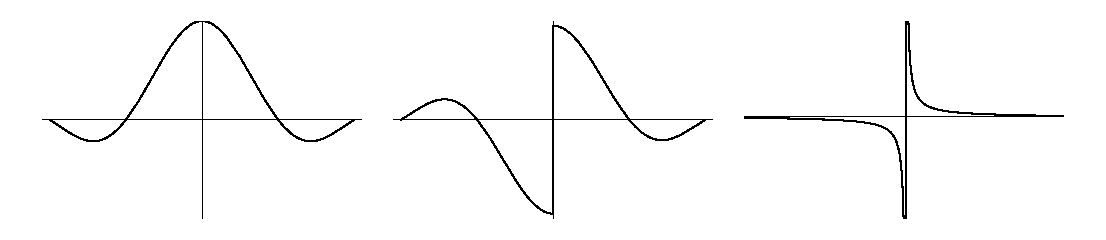
\includegraphics[height=4cm,width=10cm]{disc3.eps}
\end{center}
\end{minipage}
\caption{The functions $\frac{\sin x}{x}$, $\frac{\sin x}{|x|}$ and
    $\frac{\sin x}{1 - \cos x}$.}
\label{fig:disc3}
\label{disc3}
\end{figure}

An expression that evaluates 
(for a particular value of the independent variable)
to $\frac{0}{0}$, $\frac{\infty}{\infty}$,
$0 \cdot \infty$, $\infty - \infty$, $1^\infty$, $0^0$ or $\infty^0$
is called an \textit{indeterminate}.
A function $h(x)$ which takes an indeterminate form at $x=a$ 
is not defined for $x=a$ by the given analytical expression.
\index{indeterminate}
For example, suppose we have

\[
%\begin{smallmatrix}
y = \frac{f(x)}{g(x)},
%\end{smallmatrix}
\]
where for some value of the variable, as %x = a%,

\[
%\begin{smallmatrix}
f(a) = 0,\ \ \ \ g(a) = 0.
%\end{smallmatrix}
\]
For this value of $x$ our function is not defined and we may therefore 
assign to it any value we please. It is evident from what has gone before 
(Case II, [\S \ref{sec:18}]) that it is desirable to assign to the function a 
value that will make it continuous when $x = a$ whenever it is possible to do so.


%110. 
\section{Evaluation of a function taking on an indeterminate form}
\label{sec:110}

If when $x = a$ the function $f(x)$ assumes an indeterminate form, then

\[
%\begin{smallmatrix}
\lim_{x = a} f(x)
%\end{smallmatrix}
%[5]
\]
is taken as the value of $f(x)$ for $x = a$.
The calculation of this limiting value is called {\it evaluating the indeterminate form}.

The assumption of this limiting value makes $f(x)$ continuous for $x = a$. 
This agrees with the theorem under Case II [\S \ref{sec:18}], and also with our 
practice in Chapter \ref{ch:3}, where several functions assuming 
the indeterminate form 
$
%\begin{smallmatrix}
\frac{0}{0}
%\end{smallmatrix}
$
were evaluated. Thus, for $x = 2$ the function 
$
%\begin{smallmatrix}
\frac{x^2 - 4}{x - 2}
%\end{smallmatrix}
$ 
assumes the form 
$
%\begin{smallmatrix}
\frac{0}{0}
%\end{smallmatrix}
$
but

\[
%\begin{smallmatrix}
\lim_{x \to 2} \frac{x^2 - 4}{x - 2} = 4.
%\end{smallmatrix}
\]
Hence $4$ is taken as the value of the function for $x = 2$. 
Let us now illustrate graphically the fact that if we assume $4$ as 
the value of the function for $x = 2$, then the function is continuous for $x = 2$.
Let 
$
%\begin{smallmatrix}
y = \frac{x^2 - 4}{x - 2}
%\end{smallmatrix}
$
This equation may also be written in the form
$ y(x-2)= (x-2)(x + 2)$; or $(x-2)(y-x-2)= 0$.
Placing each factor separately equal to zero, we have
$x = 2$, and $y = x + 2$. Also, when $x = 2$, we get $y=4$.

In plotting, the loci of these equations are found to be two lines. 
Since there are infinitely many points on a line, it is clear that when 
$x = 2$, the value of $y$ (or the function) may be taken as any number 
whatever. When $x$ is different from $2$, it is seen from the 
graph of the function that the corresponding value of $y$ 
(or the function) is always found from
$y = x + 2$,
which we saw was also the limiting value of $y$ (or the function) for $x = 2$.
It is evident from geometrical considerations that if we assume $4$ 
as the value of the function for $x = 2$, then the function is continuous for $x = 2$.

Similarly, several of the examples given in Chapter \ref{ch:3} illustrate 
how the limiting values of many functions assuming indeterminate forms 
may be found by employing suitable algebraic or trigonometric transformations, 
and how in general these limiting values make the corresponding functions 
continuous at the points in question. The most general methods, however, 
for evaluating indeterminate forms depend on differentiation.

%111. 
\section{Evaluation of the indeterminate form $\frac{0}{0}$}
\label{sec:111}

Given a function of the form $\frac{f(x)}{F(x)}$ such that 
$f(a) = 0$ and $F(a) = 0$; that is, the function takes on the indeterminate 
form $\frac{0}{0}$ when $a$ is substituted for $x$. It is then required to find

\[
\lim_{x \to a} \frac{f(x)}{F(x)}.
\]
%Draw the graphs of the functions f(x) and F(x). 


\begin{figure}[h!]
%\begin{tabular}{cc}
\begin{minipage}{\textwidth}
\begin{center}
%\vspace{1.0 cm}
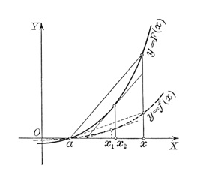
\includegraphics[height=5cm,width=6cm]{ch13-0over0form.eps}
\end{center}
\end{minipage}
\caption{The graphs of the functions $f(x)$ and $F(x)$.}
\label{fig:ch13-0over0form}
\end{figure}
Since, by hypothesis, $f(a) = 0$ and $F(a) = 0$, these graphs intersect at $(a, 0)$.

Applying the Theorem of Mean Value to each of these functions (replacing $b$ by $x$), 
we get
$f(x) = f(a) + (x-a)f'(x_1)$, $a < x_l < x$, and
$F(x) = F(a) + (x-a)F'(x_2)$. $a < x_2 < x$.
Since $f(a) = 0$ and $F(a) = 0$, we get, after canceling out $(x-a)$,

\[
\frac{f(x)}{F(x)} = \frac{f'(x_1)}{F'(x_2)}.
\]
Now let $x \to a$; then $x_l \to a$, $x_2 \to a$, and
$
\lim_{x \to a} f'(x_1) = f'(a), \lim_{x \to a} F'(x_2) = F'(a).
$
Therefore,

\begin{equation}
\label{eqn:111-49}
%(49) 	
\lim_{x \to a} \frac{f(x)}{F(x)} = \frac{f'(a)}{F'(a)},
\end{equation}
provided $F'(a) \ne 0$.
%%%%%%%%%%%%%%%%%%%%%%%%%%%%%%%%%%%
% next few examples are taken from Mauch or are my own, and not from Granville
%%%%%%%%%%%%%%%%%%%%%%%%%%%%%%%%%%%%%
This is a special case of the so-called 

\noindent
{\bf L'Hospital's Rule\footnote{Also written L'H\^opital and
pronounced ``low-peetall''.}:}
Let $f(x)$ and $F(x)$ be differentiable and $f(a) = F(a) = 0$.  
Further, let $F(x)$ be nonzero in a punctured neighborhood of $x= a$, 
(for some small $\delta$, $F(x) \neq 0$ for $x \in \{0 < |x - a| < \delta\}$).  
Then
\[
\lim_{x \to a} \frac{f(x)}{F(x)} = \lim_{x \to a} \frac{f'(x)}{F'(x)}.
\]

The rule is named after the 17th-century French mathematician 
Guillaume de l'Hospital, who published the rule in his book 
{\bf l'Analyse des Infiniment Petits pour l'Intelligence des Lignes Courbes}
(translation: Analysis of the infinitely small to understand curves) (1696), 
the first book about differential calculus, which consisted of the lectures 
of his teacher Johann Bernoulli. In particular, this rule is in fact due to
Johann Bernoulli (1667 - 1748).

\begin{example}
{\rm
  Consider the three functions $\frac{\sin x}{x}$, $\frac{\sin x}{|x|}$ and
  $\frac{\sin x}{1 - \cos x}$ at the point $x = 0$.
  \[
  \lim_{x \to 0} \frac{\sin x}{x}
  = \lim_{x \to 0} \frac{\cos x}{1} 
  = 1
  \]
  Thus $\frac{\sin x}{x}$ has a removable discontinuity at $x = 0$.
  \[
  \lim_{x \to 0^+} \frac{\sin x}{|x|}
  = \lim_{x \to 0^+} \frac{\sin x}{x} = 1
  \]
  \[
  \lim_{x \to 0^-} \frac{\sin x}{|x|}
  = \lim_{x \to 0^-} \frac{\sin x}{-x} = -1
  \]
  Thus $\frac{\sin x}{|x|}$ has a finite discontinuity at $x = 0$.
  \[
  \lim_{x \to 0} \frac{\sin x}{1 - \cos x}
  = \lim_{x \to 0} \frac{\cos x}{\sin x}
  = \frac{1}{0} = \infty
  \]
  Thus $\frac{\sin x}{1 - \cos x}$ has an infinite discontinuity at $x = 0$.
}
\end{example}

\begin{example}
{\rm
We use \sage to compute 
$\lim_{x\rightarrow 0}
\frac{\cos(x)-1}{x^2}$.

\vskip .1in

\begin{Verbatim}[fontsize=\scriptsize,fontfamily=courier,fontshape=tt,frame=single,label=\sage]

sage: limit((cos(x)-1)/x^2,x=0)
-1/2
sage: limit((-sin(x))/(2*x),x=0)
-1/2
sage: limit((-cos(x))/(2),x=0)
-1/2

\end{Verbatim}

\vskip .1in
\noindent
This verifies 

\[
\lim_{x\rightarrow 0}\frac{\cos(x)-1}{x^2}
=\lim_{x\rightarrow 0}\frac{-\sin(x)}{2x}
=\lim_{x\rightarrow 0}\frac{-\cos(x)}{2}=-1/2.
\]
}
\end{example}



\begin{example}
{\rm
  Let $a$ and $d$ be nonzero.
  \begin{align*}
    \lim_{x \to \infty} \frac{a x^2 + b x + c}{d x^2 + e x + f}
    &= \lim_{x \to \infty} \frac{2 a x + b}{2 d x + e} \\
    &= \lim_{x \to \infty} \frac{2 a}{2 d} \\
    &= \frac{a}{d}
  \end{align*}
}
\end{example}





\begin{example}
{\rm
Consider
  \[
  \lim_{x \to 0} \frac{\cos x - 1}{x \sin x}.
  \]
  This limit is an indeterminate of the form $\frac{0}{0}$.  Applying
  L'Hospital's rule we see that limit is equal to
  \[
  \lim_{x \to 0} \frac{-\sin x}{x \cos x + \sin x}.
  \]
  This limit is again an indeterminate of the form $\frac{0}{0}$.  We apply
  L'Hospital's rule again.
  \[
  \lim_{x \to 0} \frac{- \cos x}{ - x \sin x + 2 \cos x } = - \frac{1}{2}
  \]
  Thus the value of the original limit is $- \frac{1}{2}$.  We could also
  obtain this result by expanding the functions in Taylor series.
  \begin{align*}
    \lim_{x \to 0} \frac{\cos x - 1}{x \sin x}
    &= \lim_{x \to 0} \frac{\left( 1 - \frac{x^2}{2} + \frac{x^4}{24} 
        - \cdots \right) - 1 }{ x \left( x - \frac{x^3}{6} 
        + \frac{x^5}{120} - \cdots \right)} \\
    &= \lim_{x \to 0} \frac{- \frac{x^2}{2} + \frac{x^4}{24} - \cdots }
    { x^2 - \frac{x^4}{6} + \frac{x^6}{120} - \cdots } \\
    &= \lim_{x \to 0} \frac{- \frac{1}{2} + \frac{x^2}{24} - \cdots }
    { 1 - \frac{x^2}{6} + \frac{x^4}{120} - \cdots } \\
    &= - \frac{1}{2}
  \end{align*}
}
\end{example}


%%%%%%%%%%%%%%%%%%%%%%%%%%%%%%%%%%%%%%%%%%%
%% Not from Granville
%%%%%%%%%%%%%%%%%%%%%%%%%%%%%%%%%%%%%%%%%%%

\begin{example}
{\rm
We use \sage to compute 
$\lim_{x\rightarrow 0}
\frac{\cos(x)-1}{x^2}$.

\vskip .1in

\begin{Verbatim}[fontsize=\scriptsize,fontfamily=courier,fontshape=tt,frame=single,label=\sage]

sage: limit((cos(x)-1)/x^2,x=0)
-1/2
sage: limit((-sin(x))/(2*x),x=0)
-1/2
sage: limit((-cos(x))/(2),x=0)
-1/2

\end{Verbatim}

\vskip .1in
\noindent
This verifies 

\[
\lim_{x\rightarrow 0}\frac{\cos(x)-1}{x^2}
=\lim_{x\rightarrow 0}\frac{-\sin(x)}{2x}
=\lim_{x\rightarrow 0}\frac{-\cos(x)}{2}=-1/2.
\]
}
\end{example}



\subsection{Rule for evaluating the indeterminate form $\frac{0}{0}$}

Differentiate the numerator for a new numerator and the denominator 
for a new denominator\footnote{The student is warned against the very 
careless but common mistake of differentiating the whole expression as a fraction.}
The value of this new fraction for the assigned value\footnote{If 
$a = \inf$, the substitution $x = \frac{1}{z}$ reduces the problem to the 
evaluation of the limit for $z = 0$. Thus 
$\lim_{x \to \inf} \frac{f(x)}{F(x)} 
= \lim_{z \to 0} \frac{ -f' \left( \frac{1}{z} \right) 
\frac{1}{z^2} }{ -F' \left( \frac{1}{z} \right) \frac{1}{z^2} } 
= \lim_{z \to 0} \frac{f' \left( \frac{1}{z} \right)}{F' \left( \frac{1}{z} \right)} 
= \lim_{x \to \inf} \frac{f'(x)}{F'(x)}$. Therefore the rule holds in this case also.}
of the variable will be the limiting value of the original fraction.

In case it so happens that
$f'(a) = 0$ and $F'(a) = 0$,
that is, the first derivatives also vanish for $x = a$, then we 
still have the indeterminate form $\frac{0}{0}$, and the theorem can be 
applied anew to the ratio
$\frac{f'(x)}{F'(x)}$
giving us
$
\lim_{x \to a} \frac{f(x)}{F(x)} = \frac{f''(a)}{F''(a)}. 
$
When also $f''(a) = 0$ and $F''(a) = 0$, we get in the same manner
$
\lim_{x \to a} \frac{f(x)}{F(x)} = \frac{f'''(a)}{F'''(a)},
$
and so on.

It may be necessary to repeat this process several times.

\begin{example}
Evaluate $\frac{f(x)}{F(x)} = \frac{x^3 - 3x + 2}{x^3 - x^2 - x - 1}$ 
when $x = 1$.

Solution. 	

\[
\frac{f(1)}{F(1)} = \left. \frac{x^3 - 3x + 2}{x^3 - x^2 + 1} \right]_{x = 1} 
= \frac{1 - 3 + 2}{1 - 1 - 1 + 1} \ \ ``= \frac{0}{0}''.
\]
Therefore, this is an indeterminate form.

\[
\frac{f'(1)}{F'(1)} = \left. \frac{3x^2 - 3}{3x^2 - 2x - 1} \right]_{x = 1} 
= \frac{3 - 3}{3 - 2 - 1}\ \ `` = \frac{0}{0}''.
\]
Therefore, this is an indeterminate form.

\[
\frac{f''(1)}{F''(1)} = \left. \frac{6x}{6x - 2} \right]_{x = 1} 
= \frac{6}{6 - 2} = \frac{3}{2}. \ \ {\rm Ans.}
\]
\end{example}

\begin{example}
Evaluate $\lim_{x \to 0} \frac{e^x - e^{-x} - 2x}{x - \sin x}$.

Solution. 

\[
\frac{f(0)}{F(0} = \left. \frac{e^x - e^{-x} - 2x}{x - \sin x} \right]_{x = 0} 
= \frac{1 - 1 - 0}{0 - 0}\ \ `` = \frac{0}{0}''.
\]
Therefore, this is an indeterminate form.

\[
\frac{f'(0)}{F'(0)} = \left. \frac{e^x - e^{-x} - 2}{1 - \cos x} \right]_{x = 0} 
= \frac{1 + 1 - 2}{1 - 1}\ \ `` = \frac{0}{0}''.
\]
Therefore, this is an indeterminate form.

\[
\frac{f''(0)}{F''(0)} = \left. \frac{e^x - e^{-x}}{\sin x} \right]_{x = 0} 
= \frac{1 - 1}{0}\ \ `` = \frac{0}{0}''.
\]
Therefore, this is an indeterminate form.

\[
\frac{f'''(0)}{F'''(0)} = \left. \frac{e^x - e^{-x}}{\cos x} \right]_{x = 0} 
= \frac{1 + 1}{1} = 2. \ \ {\rm Ans.}
\]
\end{example}

\subsection{Exercises}

Evaluate the following by differentiation\footnote{After differentiating, 
the student should in every case reduce the resulting expression to its 
simplest possible form before substituting the value of the variable.}.

\begin{enumerate}

\item
$ \lim_{x \to 4} \frac{x^2 - 16}{x^2 + x - 20}$. 

Ans. $\frac{8}{9}$.

\item
$\lim_{x \to 1} \frac{x - 1}{x^n - 1}$. 	  

Ans. $\frac{1}{n}$.

\item
$ \lim_{x \to 1} \frac{\log x}{x - 1}$.

Ans. $1$.

\item
$\lim_{x \to 0} \frac{e^x - e^{-x}}{\sin x}$.

Ans. $2$.

\item
$\lim_{x\to 0} \frac{\tan x - x}{x - \sin x}$. 	 

Ans. $2$.

\item
$\lim_{x \to \frac{\pi}{2}} \frac{\log \sin x}{(\pi - 2x)^2}$.

Ans. $-\frac{1}{8}$.

\item
$\lim_{x \to 0} \frac{a^x - b^x}{x}$.

Ans. $\log \frac{a}{b}$.

\item
$\lim_{r \to a} \frac{r^3 - ar^2 - a^2 r + a^3}{r^2 - a^2}$.

Ans. $0$.

\item
$\lim_{\theta \to 0} \frac{\theta -\arcsin \theta}{\sin^3 \theta}$. 	

Ans. 	$-\frac{1}{6}$.

\item
$\lim_{x \to \phi} \frac{\sin x - \sin \phi}{x - \phi}$.

Ans. $\cos\phi $.

\item
$\lim_{y \to 0} \frac{e^y + \sin y - 1}{\log(1 + y)}$. 	  	

Ans. $2$.

\item
$\lim_{\theta \to 0} \frac{\tan \theta + \sec \theta -1}{\tan \theta -\sec \theta + 1}$. 

Ans. $1$.

\item
$\lim_{\phi \to \frac{\pi}{4}} \frac{\sec^2 \phi - 2 \tan \phi}{1 + \cos 4 \phi}$. 

Ans. $\frac{1}{2}$.

\item
$\lim_{z \to a} \frac{az - z^2}{a^4 - 2a^3z + 2 az^3 - z^4}$. 

Ans. $+\infty$.

\item
$\lim_{x \to 2} \frac{(e^x - e^2)^2}{(x - 4)e^x + e^2 x}$. 	  

Ans. $6e^4$.

\item
$\lim_{x \to 1} \frac{x^2 + x - 2}{x^2 - 1}$.

\item
$\lim_{x \to -2} \frac{x^3 + 8}{x^5 + 32}$.

\item
$\lim_{x \to 0} \frac{\sin 2x}{x}$.

\item
$\lim_{x \to 0} \frac{x - \sin x}{x^3}$.

\item
$\lim_{x \to 1} \frac{\log \cos (x - 1)}{1 - \sin \frac{\pi x}{2}}$.

\item
$\lim_{x \to 0} \frac{\tan x - \sin x}{\sin^3 x}$.

\end{enumerate}

%112. 
\section{Evaluation of the indeterminate form $\frac{\infty}{\infty}$}
\label{sec:112}

In order to compute

\[
  	\lim_{x \to a} \frac{f(x)}{F(x)}
\]
when $	\lim_{x \to a} f(x) = \infty$ and $\lim_{x \to a} F(x) = \infty$,
that is, when for $x = a$ the function $\frac{f(x)}{F(x)}$
assumes the indeterminate form $\frac{\infty}{\infty}$,
we follow the same rule as that given in \S \ref{sec:111} for 
evaluating the indeterminate form $\frac{0}{0}$. 

{\bf Rule for evaluating the indeterminate form $\frac{\infty}{\infty}$}:
Differentiate the numerator for a new numerator and the denominator 
for a new denominator. The value of this new fraction for the assigned 
value of the variable will be the limiting value of the original fraction.

A rigorous proof of this rule is beyond the scope of this book and is left 
for more advanced treatises.

\begin{example}
Evaluate $\frac{\log x}{\csc x}$ for $x = 0$.

Solution. 

\[
\frac{f(0)}{F(0)} = \left. \frac{\log(x)}{\csc(x)} \right]_{x = 0} 
\ \ ``= \frac{-\infty}{\infty}''. 
\]
Therefore, this is an indeterminate form.
\[
  	\frac{f'(0)}{F'(0)} = \left. \frac{\frac{1}{x}}{-\csc x \cot x} \right]_{x = 0} 
= \left. -\frac{\sin^2 x}{x \cos x} \right]_{x = 0}\ \ ``= \frac{0}{0}''.
\]
Therefore, this is an indeterminate form.
\[
  	\frac{f''(0)}{F''(0)} 
= \left. -\frac{2 \sin x \cos x}{\cos x - x \sin x} \right]_{x = 0} 
= -\frac{0}{1} = 0. \ \ {\rm Ans.}
\]

\end{example}

%%%%%%%%%%%%%%%%%%%%%%%%%%%%%%%%%%%%%%%%
% From Mauch
%%%%%%%%%%%%%%%%%%%%%%%%%%%%%%%%%%%%%%%%
\begin{example}
{\rm
  Let $a$ and $d$ be nonzero.
  \begin{align*}
    \lim_{x \to \infty} \frac{a x^2 + b x + c}{d x^2 + e x + f}
    &= \lim_{x \to \infty} \frac{2 a x + b}{2 d x + e} \\
    &= \lim_{x \to \infty} \frac{2 a}{2 d} \\
    &= \frac{a}{d}
  \end{align*}
}
\end{example}


%113. 
\section{Evaluation of the indeterminate form $0 \cdot \infty$}
\label{sec:113}

 If a function $f(x) \cdot \phi(x)$ takes on the indeterminate form 
$0 \cdot \infty$ for $x = a$, we write the given function

\[
f(x) \cdot \phi(x) = \frac{f(x)}{ \frac{1}{\phi(x)} } 
\left( \text{or} = \frac{\phi(x)}{\frac{1}{f(x)}} \right)
\]
so as to cause it to take on one of the forms $\frac{0}{0}$ or 
$\frac{\infty}{\infty}$, thus bringing it under 
\S \ref{sec:111} or \S \ref{sec:112}.

\begin{example}
Evaluate $\sec(3x)\cos(5x)$ for $x = \frac{\pi}{2}$.

Solution. $\left. \sec 3x \cos 5x \right]_{x = \frac{\pi}{2}} \ \ ``= \infty \cdot 0''$.
Therefore, this is an indeterminate form.
Substituting $\frac{1}{\cos 3x}$ for $\sec 3x$, the function 
becomes $\frac{\cos 5x}{\cos 3x} = \frac{f(x)}{F(x)}$.

\[
\frac{ f(\frac{\pi}{2}) }{ F(\frac{\pi}{2}) } 	
= \left. \frac{\cos 5x}{\cos 3x} \right]_{x = \frac{\pi}{s}}\ \ `` = \frac{0}{0}''. 
\]
Therefore, this is an indeterminate form.
\[
\frac{ f'(\frac{\pi}{2}) }{ F'(\frac{\pi}{2}) } 	
= \left. \frac{-\cos x}{- \sin x} \right]_{x = \frac{\pi}{s}} 
= \frac{0}{-1} = 0.\ \ {\rm Ans.}
\]
\end{example}

%%%%%%%%%%%%%%%%%%%%%%%%%%%%%%%%%%%%%%%%%%
%% This is an example from Mauch
%%%%%%%%%%%%%%%%%%%%%%%%%%%%%%%%%%%%%%%

\begin{example}
  \begin{align*}
    \lim_{x \to 0} \left( \cot x - \frac{1}{x} \right)
    &= \lim_{x \to 0} \frac{x \cos x - \sin x}{x \sin x} \\
    &= \lim_{x \to 0} \frac{\cos x - x \sin x - \cos x}
    {\sin x + x \cos x} \\
    &= \lim_{x \to 0} \frac{- x \sin x } {\sin x + x \cos x} \\
    &= \lim_{x \to 0} \frac{- x \cos x - \sin x } 
    {\cos x + \cos x - x \sin x } \\
    &= 0
  \end{align*}

Here is the \sage command for this example:


\vskip .1in

\begin{Verbatim}[fontsize=\scriptsize,fontfamily=courier,fontshape=tt,frame=single,label=\sage]

sage: limit(cot(x)-1/x,x=0)
0
sage: limit((- x*cos(x) - sin(x) )/(cos(x) + cos(x) - x*sin(x)),x=0)
0

\end{Verbatim}

\vskip .1in
\noindent
\end{example}

%114. 
\section{Evaluation of the indeterminate form $\infty-\infty$}
\label{sec:114}

It is possible in general to transform the expression into a fraction 
which will assume either the form $\frac{0}{0}$ or $\frac{\infty}{\infty}$.

\begin{example}
Evaluate $\sec x -\tan x$ for $x = \frac{\pi}{2}$.

Solution. 
$\left. \sec x - \tan x \right]_{x= \frac{\pi}{2}} \ \ ``= \infty - \infty''$. 
Therefore, this is an indeterminate form.
By Trigonometry, 

$\sec x - \tan x = \frac{1}{\cos x} - \frac{\sin x}{\cos x} 
= \frac{1 - \sin x}{\cos x} = \frac{f(x)}{F(x)}$.

$\frac{ f(\frac{\pi}{2}) }{ F(\frac{\pi}{2}) } 	
= \left. \frac{1 - \sin x}{\cos x} \right]_{x = \frac{\pi}{2}} 
= \frac{1 - 1}{0}\ \ `` = \frac{0}{0}''$. 
Therefore, this is an indeterminate form.

$
\frac{ f'(\frac{\pi}{2}) }{ F'(\frac{\pi}{2}) } 	
= \left. \frac{-\cos x}{-\sin x} \right]_{x = \frac{\pi}{2}} 
= \frac{0}{-1} = 0. \ \ {\rm Ans.}
$
\end{example}

\subsection{Exercises}

Evaluate the following by differentiation\footnote{In solving the remaining 
exercises in this chapter it may be of assistance to the student to 
refer to \S \ref{sec:24}, where many special forms not 
indeterminate are evaluated.}.

\begin{enumerate}

\item
$\lim_{x \to \infty} \frac{ax^2 + b}{cx^2 + d}$. 	

Ans. $\frac{a}{c}$.

\item
$\lim_{x \to 0} \frac{\cot x}{\log x}$. 

Ans. $-\infty$.

\item
$\lim_{x = \infty} \frac{\log x}{x^n}$.

Ans. $0$.

\item
$\lim_{x \to \infty} \frac{x^2}{e^x}$. 	 

Ans. $0$.

\item
$\lim_{x \to \infty} \frac{e^x}{\log x}$. 

Ans. $\infty$.

\item
$\lim_{x \to 0} x \cot \pi x$.

Ans. $\frac{1}{\pi}$.

\item
$\lim_{y \to \infty} \frac{y}{e^{ay}}$. 

Ans. $0$.

\item
$\lim_{x \to \frac{\pi}{2}} (\pi - 2x) \tan x$. 

Ans. $2$.

\item
$\lim_{x \to \infty} x \sin \frac{a}{x}$. 	  

Ans. $a$.

\item
$\lim_{x \to 0} x^n \log x$.  [$n$ positive.]

Ans. $0$.

\item
$\lim_{\theta \to \frac{\pi}{4}} (1 - \tan \theta) \sec 2\theta$.

Ans. $1$.

\item
$\lim_{\phi \to a} (a^2 - \phi^2) \tan \frac{\pi \phi}{2a}$. 

Ans. $\frac{4 a^2}{\pi}$.

\item
$\lim_{x \to 0} \frac{\log \sin 2x}{\log \sin x}$. 	

Ans. 	$1$.

\item
$\lim_{\theta \to \frac{\pi}{2}} \frac{\tan \theta}{\tan 3\theta}$. 	  	

Ans. $3$.

\item
$\lim_{\phi \to \frac{\pi}{2}} \frac{\log \left( \phi - \frac{\pi}{2} \right)}{\tan \phi}$.

Ans. $0$.

\item
$\lim_{x \to 0} \frac{\log x}{\cot x}$. 

Ans. $0$.

\item
$\lim_{x \to 0} x \log \sin x$. 

Ans. $0$.

\item
$\lim_{x \to 1} \left[ \frac{2}{x^2 - 1} - \frac{1}{x - 1} \right]$. 	

Ans. $-\frac{1}{2}$.

\vskip .1in

\begin{Verbatim}[fontsize=\scriptsize,fontfamily=courier,fontshape=tt,frame=single,label=\sage]

sage: limit(2/(x^2-1) - 1/(x-1),x=1)
-1/2

\end{Verbatim}

\item
$\lim_{x \to 1} \left[ \frac{1}{\log x} - \frac{x}{\log x} \right]$.

Ans. $-1$.
\vskip .1in

\begin{Verbatim}[fontsize=\scriptsize,fontfamily=courier,fontshape=tt,frame=single,label=\sage]

sage: limit(1/log(x) - x/log(x),x=1)
-1

\end{Verbatim}

\item
$\lim_{\theta \to \frac{\pi}{2}} [\sec \theta - \tan \theta]$. 

Ans. $0$.

\item
$\lim_{\phi \to 0} \left[ \frac{2}{\sin^2 \phi} - \frac{1}{1 - \cos \phi} \right]$.

Ans. $\frac{1}{2}$.

\item
$\lim_{y \to 1} \left[ \frac{y}{y - 1} - \frac{1}{\log y} \right]$. 

Ans. $\frac{1}{2}$.

\item
$\lim_{z \to 0} \left[ \frac{\pi}{4z} - \frac{\pi}{2z(e^{\pi z} + 1)} \right]$. 	

Ans. $\frac{\pi^2}{8}$.

\end{enumerate}


%115. 
\section{Evaluation of the indeterminate forms $0^0$, $1^{\infty}$, $\infty^0$}
\label{sec:115}

Given a function of the form

\[
  	f(x)^{\phi(x)}.
\]
In order that the function shall take on one of the above three forms, 
we must have for a certain value of $x$,
$f(x) = 0$, $\phi(x) = 0$, giving $0^0$;
or, $f(x) = 1$, $\phi(x) = \infty$, giving $1^{\infty}$;
or, $f(x) = \infty$, $\phi(x) = 0$, giving ${\infty}^0$.
Let 	$y = f(x)^{\phi(x)}$;
taking the logarithm of both sides,
  	$\log y = \phi (x)\log f(x)$.
In any of the above cases the logarithm of $y$ (the function) will take on the 
indeterminate form $0 \cdot \infty$.

Evaluating this by the process illustrated in \S \ref{sec:113} gives 
the limit of the logarithm of the function. This being equal to the 
logarithm of the limit of the function, the limit of the function is known.


\begin{example}
Evaluate $x^x$ when $x = 0$.

Solution. This function assumes the indeterminate form $0^0$ for $x = 0$.
Let $y 	=\ x^x$;
then $\log y 	= x \log x = 0 \cdot (-\infty)$, 	when $x = 0$.
By \S \ref{sec:113}, 

\[
\log y 	\frac{\log x}{\frac{1}{x}} = \frac{-\infty}{\infty}, 	
\]
when $x = 0$.
By \S \ref{sec:112},

\[
\log y 	\frac{\frac{1}{x}}{-\frac{1}{x^2}} = -x = 0,
\]
when $x = 0$.
Since $y = x^x$, this gives $\log_e(x^x) = 0$; i.e., 
$x^x = 1$. Ans.
\end{example}

\begin{example}
Evaluate $(1 + x)^{\frac{1}{x}}$ when $x = 0$.

Solution. This function assumes the indeterminate form $1^{\infty}$ for $x = 0$.
Let $y 	= (1 + x)^{\frac{1}{x}}$;
then $\log y 	= \frac{1}{x} \log(1 + x) = \infty \cdot 0$
when $x = 0$. By \S \ref{sec:113},
$ y 	= \frac{\log(1 + x)}{x} = \frac{0}{0}$, when $x = 0$.
By \S \ref{sec:111}, 
$ y 	= \frac{\frac{1}{1 + x}}{1} = \frac{1}{1 + x} = 1$
when $x = 0$.
Since $y = (1 + x)^{\frac{1}{1 + x}}$, this gives $\log_e (1 + x)^{\frac{1}{x}} = 1$; 
i.e. $(1 + x)^{\frac{1}{x}} = e$. Ans.
\end{example}

\begin{example}
Evaluate $\cot x\sin x$ for $x = 0$.

Solution. This function assumes the indeterminate form $\infty^0$ for $x = 0$.
Let $ y 	=\ (\cot x)^{\sin x}$;
then $ \log y 	=\ \sin x \log \cot x = 0 \cdot \infty$ when $x = 0$.
By \S \ref{sec:113},
$ \log y 	= \frac{\log \cot x}{\csc x} = \frac{\infty}{\infty}$
when $x = 0$.
\S \ref{sec:112},
$ \log y 	= \frac{\frac{-\csc^2 x}{\cot x}}{-\csc x \cot x} 
= \frac{\sin x}{\cos^2 x} = 0$,	when $x = 0$.
\end{example}


%%%%%%%%%%%%%%%%%%%%%%%%%%%%%%%%%%%%%%%%%%%%%
%% SOme exercises are from Mauch, some from Granville
%%%%%%%%%%%%%%%%%%%%%%%%%%%%%%%%%%%%%%%%%%%%%%%%%%%%%%%

\section{Exercises}
Evaluate the following limits.

\begin{enumerate}

\item
$\lim_{x \to 1} x^{\frac{1}{1 - x}}$. 

Ans. $\frac{1}{e}$.

\item
$\lim_{x \to 0} \left( \frac{1}{x} \right)^{\tan x}$. 

Ans. $1$.

\item
$\lim_{\theta \to \frac{\pi}{2}} (\sin \theta)^{\tan \theta}$.

Ans. $1$.

\item
$\lim_{y \to \infty} \left( 1 + \frac{a}{y} \right)^y$.

Ans. $e^a$.

\item
$\lim_{x \to 0} (1 + \sin x)^{\cot x}$. 

Ans. $e$.

\item
$\lim_{x \to \infty} \left( \frac{2}{x} + 1 \right)^x$. 

Ans. $e^2$.

\item
$\lim_{x \to 0} (e^x + x)^{\frac{1}{x}}$. 

Ans. $e^2$.

\item
$\lim_{x \to 0} (\cot x)^{\frac{1}{\log x}}$.

Ans. $\frac{1}{e}$.

\item
$\lim_{z \to 0} (1 + nz)^{\frac{1}{z}}$.

Ans. $e^n$.

\item
$\lim_{\phi \to 1} \left( \tan \frac{\pi \phi}{4} \right)^{\tan \frac{\pi \phi}{2}}$.

Ans. $\frac{1}{e}$.

\item
$\lim_{\theta \to 0} (\cos m\theta)^{\frac{n}{\theta^2}}$. 

Ans. $e^{-\frac{1}{2} nm^2}$.

\item
$\lim_{x \to 0} (\cot x)^x$. 	 

Ans. $1$.

\item
$\lim_{x \to a} \left( 2 -\frac{x}{a} \right)^{\tan \frac{\pi x}{2a}}$.

Ans. $e^{\frac{2}{\pi}}$.

\item
%1.
  %\renewcommand{\theenumi}{\alph{enumi}}
  \begin{enumerate}
  \item
    $\lim_{x \to 0} \frac{x - \sin x}{x^3}$
  \item
    $\lim_{x \to 0} \left( \csc x - \frac{1}{x} \right)$
  \item
    $\lim_{x \to +\infty} \left( 1 + \frac{1}{x} \right)^x$
  \item
    $\lim_{x \to 0} \left( \csc^2 x - \frac{1}{x^2} \right)$.
    (First evaluate using L'Hospital's rule then using a Taylor series expansion.
    You will find that the latter method is more convenient.)
  \end{enumerate}
%  \renewcommand{\theenumi}{\arabic{enumi}}

%  \ifthenelse{\boolean{online}}
%  {
%    \noindent
%    \hyperref[hint lim (x - sin x)/x3]{Hint},
%    \hyperref[solution lim (x - sin x)/x3]{Solution}
%    }
%  {
%    }

\item
%2.
  \[
  \lim_{x \to \infty} x^{a/x}, \qquad
  \lim_{x \to \infty} \left( 1 + \frac{a}{x} \right)^{b x},
  \]
  where $a$ and $b$ are constants.

%  \ifthenelse{\boolean{online}}
%  {
%    \noindent
%    \hyperref[hint lim x a/x]{Hint},
%    \hyperref[solution lim x a/x]{Solution}
%    }
%  {
%    }

%3
\item
$\lim_{x \to 4}\frac{x^2-16}{x^2+x-20}$

Ans. $8/9$

%4
\item
$\lim_{x \to 1}\frac{x-1}{x^n-1}$.

Ans. $1/n$

%5
\item
$\lim_{x \to 1} \frac{\log x}{x-1}$.

Ans. $1$

%6
\item
$\lim_{x \to 0} \frac{e^x-e^{-x}}{\sin(x)}$

Ans. $2$

%7
\item
$\lim_{x \to \pi/2} \frac{\log\,\sin(x)}{(\pi-2x)^2}$

Ans. $-1/8$

%8
\item
$\lim_{x \to 0} \frac{a^x-b^x}{x}$

Ans. $\log(a/b)$

%9
\item
$\lim_{x \to 0} \frac{\theta -\arcsin(\theta)}{\theta^2}$

Ans. $-1/6$.

%10
\item
$\lim_{x \to \phi} \frac{\sin(x)-\sin(\phi)}{x-\phi}$.

Ans. $\cos(\phi)$.



\end{enumerate}

